% answers.tex —— 2007 年·普通高等学校招生考试·新课标卷·理科 · 参考答案与详细解析片段
% 由 tools/generate_projects.py 依来源总账自 2007/2007_数学真题_新课标理_试题.md + 2007/2007_数学真题_新课标理_解析正文.md + 2007/2007_数学真题_新课标理_答案要点.md 生成，勿手改（改源 MD 后重跑）


\begin{gktip}
固定候选 PDF 仅含题面，无答案、解析和评分标准，原卷亦未标注分值；以下为非官方编者独立推导，官方答案字段为空。来源发布者、出版者、版次与官方身份均未核。
\end{gktip}

\begin{answer}
\gksolhead{1}{}

\textbf{题目}：

已知命题 $p$：$\forall x\in\mathbf R$，$\sin x\leqslant1$，则（　）

（A）$\neg p$：$\exists x\in\mathbf R$，$\sin x\geqslant1$

（B）$\neg p$：$\forall x\in\mathbf R$，$\sin x\geqslant1$

（C）$\neg p$：$\exists x\in\mathbf R$，$\sin x>1$

（D）$\neg p$：$\forall x\in\mathbf R$，$\sin x>1$

\Needspace{4\baselineskip}
\textbf{解析}

\Needspace{5\baselineskip}
全称命题的否定，先把全称量词改为存在量词，再否定结论：

\nopagebreak[4]
\[\neg p:\ \exists x\in\mathbf R,\ \sin x>1.\]

原命题的结论是 $\sin x\leqslant1$，其否定为 $\sin x>1$，不是 $\sin x\geqslant1$。故选 C。

（判断要点：全称命题的否定是存在命题，且不等号要取反方向；$\leqslant$ 的否定是 $>$，不是 $\geqslant$。）

\gkanswer{答案：C。}

\end{answer}
\begin{answer}
\gksolhead{2}{}

\textbf{题目}：

已知平面向量 $\boldsymbol a=(1,1)$，$\boldsymbol b=(1,-1)$，则向量 $\dfrac12\boldsymbol a-\dfrac32\boldsymbol b=$（　）

（A）$(-2,-1)$

（B）$(-2,1)$

（C）$(-1,0)$

（D）$(-1,2)$

\Needspace{4\baselineskip}
\textbf{解析}

\nopagebreak[4]
\[\frac12\boldsymbol a=\left(\frac12,\frac12\right),\qquad \frac32\boldsymbol b=\left(\frac32,-\frac32\right),\]

\Needspace{5\baselineskip}
相减：

\nopagebreak[4]
\[\frac12\boldsymbol a-\frac32\boldsymbol b=\left(\frac12-\frac32,\frac12+\frac32\right)=(-1,2),\]

选 D。

（判断要点：$\boldsymbol b=(1,-1)$ 乘以 $\dfrac32$ 后第二分量是 $-\dfrac32$，再作差时负负得正。）

\gkanswer{答案：D。}

\end{answer}
\begin{answer}
\gksolhead{3}{}

\textbf{题目}：

函数 $y=\sin\left(2x-\dfrac{\pi}{3}\right)$ 在区间 $\left[-\dfrac{\pi}{2},\pi\right]$ 的简图是（　）
\nopagebreak[4]
\begin{center}% 2007 年新课标卷理科第 3 题：函数 y=sin(2x-π/3) 在 [-π/2,π] 上的四个简图选项。
%   （A）为正确图象；（B）（C）（D）为相位不同的干扰项。
% 来源 PDF：gaokaomath-src/普通高考/2007/2007新课标理(海南,宁夏).pdf
% SHA-256：c8ee1632ac3a7a28aab1150f047a2e1c74398ca2944701e9165237897ae724e2
% 原页：2007新课标理(海南,宁夏).pdf 第 1 页（A3 三栏）第 1 栏，书页码 393。
% 重绘依据：按原页四个小图的零点、极值位置与坐标轴标注重绘；横轴以 π 为单位。
\begin{tikzpicture}[x=2.6cm, y=1.6cm, semithick,
  every node/.style={inner sep=1pt, font=\small}]

  % ================= （A）正确图象 =================
  \begin{scope}[shift={(0cm,0cm)}]
    \draw[->,>=stealth] (-0.66,0) -- (1.20,0) node[right] {$x$};
    \draw[->,>=stealth] (0,-1.22) -- (0,1.38) node[above] {$y$};
    \draw[domain=-0.5:1,samples=200,line width=1pt]
      plot (\x,{sin(deg(2*pi*\x - pi/3))});
    \draw[dashed] (-0.5,0) -- (-0.5,{sin(deg(-pi - pi/3))});
    \draw[dashed] (1,0) -- (1,{sin(deg(2*pi - pi/3))});
    \node[below] at (-0.5,0) {$-\frac{\pi}{2}$};
    \node[below left=1pt] at (0,0) {$O$};
    \node[below] at (1,0) {$\pi$};
    \node[left=2pt] at (0,1) {$1$};
    \node[left=2pt] at (0,-1) {$-1$};
    \node[below] at (0.55,-1.55) {（A）};
  \end{scope}

  % ================= （B） =================
  \begin{scope}[shift={(7.2cm,0cm)}]
    \draw[->,>=stealth] (-0.66,0) -- (1.20,0) node[right] {$x$};
    \draw[->,>=stealth] (0,-1.22) -- (0,1.38) node[above] {$y$};
    \draw[domain=-0.5:1,samples=200,line width=1pt]
      plot (\x,{sin(deg(2*pi*\x + pi/3))});
    \draw[dashed] (-0.5,0) -- (-0.5,{sin(deg(-pi + pi/3))});
    \draw[dashed] (1,0) -- (1,{sin(deg(2*pi + pi/3))});
    \node[below] at (-0.5,0) {$-\frac{\pi}{2}$};
    \node[below left=1pt] at (0,0) {$O$};
    \node[below] at (1,0) {$\pi$};
    \node[left=2pt] at (0,1) {$1$};
    \node[left=2pt] at (0,-1) {$-1$};
    \node[below] at (0.55,-1.55) {（B）};
  \end{scope}

  % ================= （C） =================
  \begin{scope}[shift={(0cm,-5.35cm)}]
    \draw[->,>=stealth] (-0.66,0) -- (1.20,0) node[right] {$x$};
    \draw[->,>=stealth] (0,-1.22) -- (0,1.38) node[above] {$y$};
    \draw[domain=-0.5:1,samples=200,line width=1pt]
      plot (\x,{sin(deg(2*pi*\x - 2*pi/3))});
    \draw[dashed] (-0.5,0) -- (-0.5,{sin(deg(-pi - 2*pi/3))});
    \draw[dashed] (1,0) -- (1,{sin(deg(2*pi - 2*pi/3))});
    \node[below] at (-0.5,0) {$-\frac{\pi}{2}$};
    \node[below left=1pt] at (0,0) {$O$};
    \node[below] at (1,0) {$\pi$};
    \node[left=2pt] at (0,1) {$1$};
    \node[left=2pt] at (0,-1) {$-1$};
    \node[below] at (0.55,-1.55) {（C）};
  \end{scope}

  % ================= （D） =================
  \begin{scope}[shift={(7.2cm,-5.35cm)}]
    \draw[->,>=stealth] (-0.66,0) -- (1.20,0) node[right] {$x$};
    \draw[->,>=stealth] (0,-1.22) -- (0,1.38) node[above] {$y$};
    \draw[domain=-0.5:1,samples=200,line width=1pt]
      plot (\x,{sin(deg(2*pi*\x + 2*pi/3))});
    \draw[dashed] (-0.5,0) -- (-0.5,{sin(deg(-pi + 2*pi/3))});
    \draw[dashed] (1,0) -- (1,{sin(deg(2*pi + 2*pi/3))});
    \node[below] at (-0.5,0) {$-\frac{\pi}{2}$};
    \node[below left=1pt] at (0,0) {$O$};
    \node[below] at (1,0) {$\pi$};
    \node[left=2pt] at (0,1) {$1$};
    \node[left=2pt] at (0,-1) {$-1$};
    \node[below] at (0.55,-1.55) {（D）};
  \end{scope}
\end{tikzpicture}
\end{center}
\nopagebreak[4]
\Needspace{4\baselineskip}
\textbf{解析}

\Needspace{5\baselineskip}
求零点：

\nopagebreak[4]
\[2x-\frac{\pi}{3}=k\pi\ \Rightarrow\ x=\frac{\pi}{6}+\frac{k\pi}{2}.\]

\Needspace{5\baselineskip}
在 $\left[-\dfrac{\pi}{2},\pi\right]$ 内取 $k=-1,0,1,2$：

\nopagebreak[4]
\[x=-\frac{\pi}{3},\quad \frac{\pi}{6},\quad \frac{2\pi}{3},\quad \frac{7\pi}{6}.\]

其中 $\dfrac{7\pi}{6}>\pi$，舍去，故零点为 $-\dfrac{\pi}{3}$，$\dfrac{\pi}{6}$，$\dfrac{2\pi}{3}$。

\Needspace{5\baselineskip}
再取端点与特殊点：

\nopagebreak[4]
\[x=-\frac{\pi}{2}:\ y=\sin\left(-\pi-\frac{\pi}{3}\right)=\frac{\sqrt3}{2}>0,\]

\nopagebreak[4]
\[x=0:\ y=\sin\left(-\frac{\pi}{3}\right)=-\frac{\sqrt3}{2}<0,\]

\nopagebreak[4]
\[x=\pi:\ y=\sin\left(2\pi-\frac{\pi}{3}\right)=-\frac{\sqrt3}{2}<0.\]

图象应从 $-\dfrac{\pi}{2}$ 处的正值下降，经过 $-\dfrac{\pi}{3}$ 变号，在 $x=-\dfrac{\pi}{12}$ 附近取最小值 $-1$，再经过 $\dfrac{\pi}{6}$ 上升，在 $x=\dfrac{5\pi}{12}$ 附近取最大值 $1$，最后经过 $\dfrac{2\pi}{3}$ 下降。与四个选项比对，只有（A）满足。选 A。

（判断要点：先解出区间内的全部零点，再用 $x=0$、端点处的函数值定符号；最大值的横坐标 $\dfrac{5\pi}{12}$ 在 $\dfrac{\pi}{6}$ 与 $\dfrac{\pi}{2}$ 之间。）

\gkanswer{答案：A。}

\end{answer}
\begin{answer}
\gksolhead{4}{}

\textbf{题目}：

已知 $\{a_n\}$ 是等差数列，$a_{10}=10$，其前 $10$ 项和 $S_{10}=70$，则其公差 $d=$（　）

（A）$-\dfrac23$

（B）$-\dfrac13$

（C）$\dfrac13$

（D）$\dfrac23$

\Needspace{4\baselineskip}
\textbf{解析}

\Needspace{5\baselineskip}
等差数列前 $n$ 项和与通项分别为

\nopagebreak[4]
\[S_{10}=10a_1+\frac{10\times9}{2}d=10a_1+45d=70,\]

\nopagebreak[4]
\[a_{10}=a_1+9d=10.\]

\Needspace{5\baselineskip}
由第二式得 $a_1=10-9d$，代入第一式：

\nopagebreak[4]
\[10(10-9d)+45d=70\ \Rightarrow\ 100-45d=70\ \Rightarrow\ d=\frac23.\]

选 D。

（判断要点：两个条件对应两个方程，先消去 $a_1$ 求 $d$；$S_{10}$ 的系数是 $\dfrac{10\times9}{2}=45$，不要误写成 $55$。）

\gkanswer{答案：D。}

\end{answer}
\begin{answer}
\gksolhead{5}{}

\textbf{题目}：

如果执行下面的程序框图，那么输出的 $S=$（　）
\nopagebreak[4]
\begin{center}% 2007 年新课标卷理科第 5 题：程序框图（k 从 1 到 50 累加 2k）。
% 来源 PDF：gaokaomath-src/普通高考/2007/2007新课标理(海南,宁夏).pdf
% SHA-256：c8ee1632ac3a7a28aab1150f047a2e1c74398ca2944701e9165237897ae724e2
% 原页：2007新课标理(海南,宁夏).pdf 第 1 页（A3 三栏）第 1 栏，书页码 393。
% 重绘依据：按原页流程与分支方向重绘；循环体为 S=S+2k、k=k+1。
\begin{tikzpicture}[scale=1.0, semithick,
  every node/.style={inner sep=2pt},
  box/.style={draw, rounded corners=2pt, minimum width=1.9cm,
    minimum height=0.55cm, align=center},
  para/.style={draw, trapezium, trapezium left angle=70,
    trapezium right angle=110, minimum width=2.4cm, minimum height=0.55cm,
    align=center},
  dec/.style={draw, diamond, aspect=2.4, minimum width=2.8cm,
    minimum height=1.1cm, align=center},
  arr/.style={->, >=stealth}]

  \node[box]  (start) at (0,7.2) {开始};
  \node[box]  (init)  at (0,6.3) {$k=1$};
  \node[box]  (sum)   at (0,5.4) {$S=0$};
  \node[dec]  (test)  at (0,4.2) {$k\leqslant50$?};
  \node[box]  (add)   at (0,2.95) {$S=S+2k$};
  \node[box]  (inc)   at (0,2.15) {$k=k+1$};
  \node[para] (out)   at (4.6,4.2) {输出 $S$};
  \node[box]  (end)   at (4.6,3.3) {结束};

  \draw[arr] (start) -- (init);
  \draw[arr] (init) -- (sum);
  \draw[arr] (sum) -- (test);
  \draw[arr] (test.south) -- node[left] {是} (add.north);
  \draw[arr] (add) -- (inc);
  \draw[arr] (inc.west) -- (-2.5,2.15) -- (-2.5,4.75) -- (0,4.75);
  \draw[arr] (test.east) -- node[above] {否} (out.west);
  \draw[arr] (out) -- (end);
\end{tikzpicture}
\end{center}
\nopagebreak[4]
（A）$2450$

（B）$2500$

（C）$2550$

（D）$2652$

\Needspace{4\baselineskip}
\textbf{解析}

\Needspace{5\baselineskip}
初始 $k=1$，$S=0$。每次判断 $k\leqslant50$，成立则执行

\nopagebreak[4]
\[S=S+2k,\qquad k=k+1.\]

\Needspace{5\baselineskip}
故循环把 $2\times1,2\times2,\cdots,2\times50$ 依次加入 $S$：

\nopagebreak[4]
\[S=2(1+2+\cdots+50)=2\times\frac{50\times51}{2}=2550.\]

选 C。

（判断要点：循环变量从 $1$ 到 $50$，共 $50$ 项；$1+2+\cdots+50=1275$，乘 $2$ 得 $2550$。）

\gkanswer{答案：C。}

\end{answer}
\begin{answer}
\gksolhead{6}{}

\textbf{题目}：

已知抛物线 $y^2=2px$（$p>0$）的焦点为 $F$，点 $P_1(x_1,y_1)$，$P_2(x_2,y_2)$，$P_3(x_3,y_3)$ 在抛物线上，且 $2x_2=x_1+x_3$，则有（　）

（A）$|FP_1|+|FP_2|=|FP_3|$

（B）$|FP_1|^2+|FP_2|^2=|FP_3|^2$

（C）$2|FP_2|=|FP_1|+|FP_3|$

（D）$|FP_2|^2=|FP_1|\cdot|FP_3|$

\Needspace{4\baselineskip}
\textbf{解析}

\Needspace{5\baselineskip}
抛物线 $y^2=2px$ 的准线为 $x=-\dfrac p2$，焦半径公式为

\nopagebreak[4]
\[|FP|=x+\frac p2.\]

\Needspace{5\baselineskip}
由 $2x_2=x_1+x_3$，两边同时加 $p$：

\nopagebreak[4]
\[2x_2+p=x_1+x_3+p,\]

\Needspace{5\baselineskip}
即

\nopagebreak[4]
\[2\left(x_2+\frac p2\right)=\left(x_1+\frac p2\right)+\left(x_3+\frac p2\right).\]

\Needspace{5\baselineskip}
故

\nopagebreak[4]
\[2|FP_2|=|FP_1|+|FP_3|,\]

选 C。

（判断要点：抛物线上的点到焦点的距离等于到准线的距离，焦半径是 $x+\dfrac p2$；条件 $2x_2=x_1+x_3$ 是横坐标的等差关系，加 $p$ 后仍保持等差。）

\gkanswer{答案：C。}

\end{answer}
\begin{answer}
\gksolhead{7}{}

\textbf{题目}：

已知 $x>0$，$y>0$，$x$，$a$，$b$，$y$ 成等差数列，$x$，$c$，$d$，$y$ 成等比数列，则 $\dfrac{(a+b)^2}{cd}$ 的最小值是（　）

（A）$0$

（B）$1$

（C）$2$

（D）$4$

\Needspace{4\baselineskip}
\textbf{解析}

\Needspace{5\baselineskip}
$x$，$a$，$b$，$y$ 成等差数列，设公差为 $d$，则

\nopagebreak[4]
\[a=x+d,\qquad b=x+2d,\qquad y=x+3d.\]

\Needspace{5\baselineskip}
于是

\nopagebreak[4]
\[a+b=2x+3d=x+(x+3d)=x+y.\]

\Needspace{5\baselineskip}
$x$，$c$，$d$，$y$ 成等比数列，设公比为 $q$，则

\nopagebreak[4]
\[c=xq,\qquad d=xq^2,\qquad y=xq^3,\]

\Needspace{5\baselineskip}
故

\nopagebreak[4]
\[cd=x^2q^3=xy.\]

\Needspace{5\baselineskip}
因此

\nopagebreak[4]
\[\frac{(a+b)^2}{cd}=\frac{(x+y)^2}{xy}.\]

\Needspace{5\baselineskip}
由基本不等式，

\nopagebreak[4]
\[\frac{(x+y)^2}{xy}=\frac{x^2+2xy+y^2}{xy}=\frac xy+2+\frac yx\geqslant2+2=4,\]

等号当 $x=y$ 时成立。最小值为 $4$，选 D。

（判断要点：等差数列中首尾两项之和等于中间两项之和；等比数列中 $cd=xy$；最后用 $\dfrac xy+\dfrac yx\geqslant2$。）

\gkanswer{答案：D。}

\end{answer}
\begin{answer}
\gksolhead{8}{}

\textbf{题目}：

已知某个几何体的三视图如下，根据图中标出的尺寸（单位：$\mathrm{cm}$），可得这个几何体的体积是（　）
\nopagebreak[4]
\begin{center}% 2007 年新课标卷理科第 8 题：三视图（正视图、侧视图、俯视图）及尺寸。
%   正视图为直角边 20、20 的直角三角形；侧视图为底边 20、高 20 的等腰三角形；
%   俯视图为 20×20 正方形并画对角线，右侧标注 10 与 10。
% 来源 PDF：gaokaomath-src/普通高考/2007/2007新课标理(海南,宁夏).pdf
% SHA-256：c8ee1632ac3a7a28aab1150f047a2e1c74398ca2944701e9165237897ae724e2
% 原页：2007新课标理(海南,宁夏).pdf 第 1 页（A3 三栏）第 2 栏，书页码 393。
% 重绘依据：按原页三个视图的位置、形状与尺寸标注重绘，单位 cm。
\begin{tikzpicture}[x=0.115cm, y=0.095cm, semithick,
  every node/.style={inner sep=1.5pt, font=\small}]

  % ---------------- 正视图 ----------------
  \begin{scope}[shift={(0cm,0cm)}]
    \draw (0,0) -- (20,0) -- (20,20) -- cycle;
    % 尺寸 20（下）
    \draw[<->,>=stealth] (0,-4) -- (20,-4);
    \draw (0,-1.5) -- (0,-5.5);
    \draw (20,-1.5) -- (20,-5.5);
    \node[below] at (10,-4) {$20$};
    % 尺寸 20（右）
    \draw[<->,>=stealth] (24,0) -- (24,20);
    \draw (22,0) -- (26,0);
    \draw (22,20) -- (26,20);
    \node[right] at (24,10) {$20$};
    \node[below] at (10,-9) {正视图};
  \end{scope}

  % ---------------- 侧视图 ----------------
  \begin{scope}[shift={(3.6cm,0cm)}]
    \draw (0,0) -- (20,0) -- (10,20) -- cycle;
    \draw[<->,>=stealth] (0,-4) -- (20,-4);
    \draw (0,-1.5) -- (0,-5.5);
    \draw (20,-1.5) -- (20,-5.5);
    \node[below] at (10,-4) {$20$};
    \node[below] at (10,-9) {侧视图};
  \end{scope}

  % ---------------- 俯视图 ----------------
  \begin{scope}[shift={(0.9cm,-3.6cm)}]
    \draw (0,0) rectangle (20,20);
    \draw (0,0) -- (20,20);
    \draw (0,20) -- (20,0);
    % 尺寸 20（下）
    \draw[<->,>=stealth] (0,-4) -- (20,-4);
    \draw (0,-1.5) -- (0,-5.5);
    \draw (20,-1.5) -- (20,-5.5);
    \node[below] at (10,-4) {$20$};
    % 右侧 10 与 10
    \draw[<->,>=stealth] (24,0) -- (24,10);
    \draw[<->,>=stealth] (24,10) -- (24,20);
    \draw (22,0) -- (26,0);
    \draw (22,10) -- (26,10);
    \draw (22,20) -- (26,20);
    \node[right] at (24,5) {$10$};
    \node[right] at (24,15) {$10$};
    \node[below] at (10,-9) {俯视图};
  \end{scope}
\end{tikzpicture}
\end{center}
\nopagebreak[4]
（A）$\dfrac{4000}{3}\ \mathrm{cm^3}$

（B）$\dfrac{8000}{3}\ \mathrm{cm^3}$

（C）$2000\ \mathrm{cm^3}$

（D）$4000\ \mathrm{cm^3}$

\Needspace{4\baselineskip}
\textbf{解析}

由三视图还原几何体：正视图是直角边为 $20$ 的直角三角形，侧视图是底边 $20$、高 $20$ 的等腰三角形，俯视图是边长为 $20$ 的正方形（带两条对角线）。这对应一个底面为 $20\times20$ 正方形、高为 $20$ 的四棱锥（顶点在底面一条边的中点正上方，故正视图为直角三角形、侧视图为等腰三角形）。

\Needspace{5\baselineskip}
体积

\nopagebreak[4]
\[V=\frac13Sh=\frac13\times20^2\times20=\frac{8000}{3}\ \mathrm{cm^3}.\]

选 B。

（判断要点：三视图给出底面是正方形、高为 $20$；四棱锥体积是 $\dfrac13$ 底面积乘高，不要漏掉 $\dfrac13$。）

\gkanswer{答案：B。}

\end{answer}
\begin{answer}
\gksolhead{9}{}

\textbf{题目}：

若 $\dfrac{\cos2\alpha}{\sin\left(\alpha-\dfrac{\pi}{4}\right)}=-\dfrac{\sqrt2}{2}$，则 $\cos\alpha+\sin\alpha$ 的值为（　）

（A）$-\dfrac{\sqrt7}{2}$

（B）$-\dfrac12$

（C）$\dfrac12$

（D）$\dfrac{\sqrt7}{2}$

\Needspace{4\baselineskip}
\textbf{解析}

\Needspace{5\baselineskip}
利用和差公式与二倍角公式：

\nopagebreak[4]
\[\sin\left(\alpha-\frac{\pi}{4}\right)=\frac{\sqrt2}{2}(\sin\alpha-\cos\alpha)=\frac{\sin\alpha-\cos\alpha}{\sqrt2},\]

\nopagebreak[4]
\[\cos2\alpha=\cos^2\alpha-\sin^2\alpha=(\cos\alpha-\sin\alpha)(\cos\alpha+\sin\alpha).\]

\Needspace{5\baselineskip}
代入原式：

\nopagebreak[4]
\[\frac{(\cos\alpha-\sin\alpha)(\cos\alpha+\sin\alpha)}{\frac{1}{\sqrt2}(\sin\alpha-\cos\alpha)}=-\sqrt2(\cos\alpha+\sin\alpha).\]

\Needspace{5\baselineskip}
由已知它等于 $-\dfrac{\sqrt2}{2}$，故

\nopagebreak[4]
\[\cos\alpha+\sin\alpha=\frac12.\]

选 C。

（判断要点：$\cos2\alpha$ 分解为 $(\cos\alpha-\sin\alpha)(\cos\alpha+\sin\alpha)$，与分母中的 $\sin\alpha-\cos\alpha$ 约去后只剩一个负号；不要漏掉 $\sqrt2$。）

\gkanswer{答案：C。}

\end{answer}
\begin{answer}
\gksolhead{10}{}

\textbf{题目}：

曲线 $y=\mathrm e^{\frac12x}$ 在点 $(4,\mathrm e^2)$ 处的切线与坐标轴所围三角形的面积为（　）

（A）$\dfrac92\mathrm e^2$

（B）$4\mathrm e^2$

（C）$2\mathrm e^2$

（D）$\mathrm e^2$

\Needspace{4\baselineskip}
\textbf{解析}

\nopagebreak[4]
\[y=\mathrm e^{x/2},\qquad y'=\frac12\mathrm e^{x/2}.\]

\Needspace{5\baselineskip}
在 $x=4$ 处，$y=\mathrm e^2$，斜率

\nopagebreak[4]
\[k=\frac12\mathrm e^2.\]

\Needspace{5\baselineskip}
切线方程：

\nopagebreak[4]
\[y-\mathrm e^2=\frac{\mathrm e^2}{2}(x-4),\]

\Needspace{5\baselineskip}
即

\nopagebreak[4]
\[y=\frac{\mathrm e^2}{2}x-\mathrm e^2.\]

\Needspace{5\baselineskip}
令 $y=0$ 得 $x=2$；令 $x=0$ 得 $y=-\mathrm e^2$。切线与两坐标轴围成的三角形两直角边长分别为 $2$ 与 $\mathrm e^2$，面积

\nopagebreak[4]
\[S=\frac12\times2\times\mathrm e^2=\mathrm e^2.\]

选 D。

（判断要点：先求导得斜率 $\dfrac12\mathrm e^2$，再写点斜式；截距一个在 $x$ 轴正半轴、一个在 $y$ 轴负半轴，面积取长度乘积的一半。）

\gkanswer{答案：D。}

\end{answer}
\begin{answer}
\gksolhead{11}{}

\textbf{题目}：

甲、乙、丙三名射箭运动员在某次测试中各射箭 $20$ 次，三人的测试成绩如下表

\begin{center}
\begin{tabular}{llllll}
\toprule
运动员 & 环数 & $7$ & $8$ & $9$ & $10$ \\
\midrule
甲 & 频数 & $5$ & $5$ & $5$ & $5$ \\
乙 & 频数 & $6$ & $4$ & $4$ & $6$ \\
丙 & 频数 & $4$ & $6$ & $6$ & $4$ \\
\bottomrule
\end{tabular}
\end{center}

$s_1$，$s_2$，$s_3$ 分别表示甲、乙、丙三名运动员这次测试成绩的标准差，则有（　）

（A）$s_3>s_1>s_2$

（B）$s_2>s_1>s_3$

（C）$s_1>s_2>s_3$

（D）$s_2>s_3>s_1$

\Needspace{4\baselineskip}
\textbf{解析}

\Needspace{5\baselineskip}
三人的平均成绩都为

\nopagebreak[4]
\[\bar x=\frac{7+8+9+10}{4}=8.5.\]

\Needspace{5\baselineskip}
方差分别为

\nopagebreak[4]
\[s_1^2=\frac{(7-8.5)^2+(8-8.5)^2+(9-8.5)^2+(10-8.5)^2}{4}=1.25,\]

\nopagebreak[4]
\[s_2^2=\frac{6(7-8.5)^2+4(8-8.5)^2+4(9-8.5)^2+6(10-8.5)^2}{20}=1.45,\]

\nopagebreak[4]
\[s_3^2=\frac{4(7-8.5)^2+6(8-8.5)^2+6(9-8.5)^2+4(10-8.5)^2}{20}=1.05.\]

\Needspace{5\baselineskip}
故

\nopagebreak[4]
\[s_2>s_1>s_3,\]

选 B。

（判断要点：三人平均数相同，只需比较方差；乙在两端的人数最多、丙在中间的人数最多，故乙最分散、丙最集中。）

\gkanswer{答案：B。}

\end{answer}
\begin{answer}
\gksolhead{12}{}

\textbf{题目}：

一个四棱锥和一个三棱锥恰好可以拼接成一个三棱柱，这个四棱锥的底面为正方形，且底面边长与各侧棱长相等，这个三棱锥的底面边长与各侧棱长都相等。设四棱锥、三棱锥、三棱柱的高分别为 $h_1$，$h_2$，$h$，则 $h_1:h_2:h=$（　）

（A）$\sqrt3:1:1$

（B）$\sqrt3:2:2$

（C）$\sqrt3:2:\sqrt2$

（D）$\sqrt3:2:\sqrt3$

\Needspace{4\baselineskip}
\textbf{解析}

设四棱锥与正三棱锥的公共边长为 $a$。

\Needspace{5\baselineskip}
四棱锥底面为边长 $a$ 的正方形，侧棱长也为 $a$。顶点在底面中心正上方，底面中心到顶点距离为 $\dfrac{a}{\sqrt2}$，故

\nopagebreak[4]
\[h_1=\sqrt{a^2-\left(\frac{a}{\sqrt2}\right)^2}=\frac{a}{\sqrt2}.\]

\Needspace{5\baselineskip}
正三棱锥（正四面体）高为

\nopagebreak[4]
\[h_2=\sqrt{a^2-\left(\frac{\sqrt3}{3}a\right)^2}=\frac{\sqrt6}{3}a.\]

\Needspace{5\baselineskip}
两部分体积之和等于三棱柱体积。四棱锥体积为 $\dfrac13a^2h_1$，正四面体体积为 $\dfrac13\cdot\dfrac{\sqrt3}{4}a^2h_2$，三棱柱体积为 $\dfrac{\sqrt3}{4}a^2h$，故

\nopagebreak[4]
\[\frac13a^2\cdot\frac{a}{\sqrt2}+\frac13\cdot\frac{\sqrt3}{4}a^2\cdot\frac{\sqrt6}{3}a=\frac{\sqrt3}{4}a^2h.\]

\Needspace{5\baselineskip}
化简左边：

\nopagebreak[4]
\[\frac{a^3}{3\sqrt2}+\frac{\sqrt2}{12}a^3=\frac{2\sqrt2+\sqrt2}{12}a^3=\frac{\sqrt2}{4}a^3.\]

\Needspace{5\baselineskip}
于是

\nopagebreak[4]
\[\frac{\sqrt2}{4}a^3=\frac{\sqrt3}{4}a^2h\ \Rightarrow\ h=\frac{\sqrt6}{3}a.\]

\Needspace{5\baselineskip}
故

\nopagebreak[4]
\[h_1:h_2:h=\frac{a}{\sqrt2}:\frac{\sqrt6}{3}a:\frac{\sqrt6}{3}a=\sqrt3:2:2.\]

选 B。

（判断要点：四棱锥高用底面中心到顶点的距离 $\dfrac{a}{\sqrt2}$；正四面体高为 $\dfrac{\sqrt6}{3}a$；用体积和求三棱柱高，再统一比例。）

\gkanswer{答案：B。}

\end{answer}
\begin{answer}
\gksolhead{13}{}

\textbf{题目}：

已知双曲线的顶点到渐近线的距离为 $2$，焦点到渐近线的距离为 $6$，则该双曲线的离心率为\gkblank{}。

\Needspace{4\baselineskip}
\textbf{解析}

\Needspace{5\baselineskip}
设双曲线为

\nopagebreak[4]
\[\frac{x^2}{a^2}-\frac{y^2}{b^2}=1,\]

渐近线为 $bx-ay=0$，即 $bx-ay=0$。

\Needspace{5\baselineskip}
顶点 $(a,0)$ 到渐近线的距离：

\nopagebreak[4]
\[d_1=\frac{|ba|}{\sqrt{a^2+b^2}}=\frac{ab}{c}=2.\]

\Needspace{5\baselineskip}
焦点 $(c,0)$ 到渐近线的距离：

\nopagebreak[4]
\[d_2=\frac{|bc|}{\sqrt{a^2+b^2}}=b=6.\]

\Needspace{5\baselineskip}
由 $b=6$ 与 $\dfrac{ab}{c}=2$ 得

\nopagebreak[4]
\[\frac{6a}{c}=2\ \Rightarrow\ c=3a,\]

\Needspace{5\baselineskip}
故离心率

\nopagebreak[4]
\[e=\frac ca=3.\]

（判断要点：双曲线焦点到渐近线的距离恰为 $b$，这是常用结论；顶点到渐近线的距离为 $\dfrac{ab}{c}$。）

\gkanswer{答案：$3$。}

\end{answer}
\begin{answer}
\gksolhead{14}{}

\textbf{题目}：

设函数 $f(x)=\dfrac{(x+1)(x+a)}{x}$ 为奇函数，则 $a=$\gkblank{}。

\Needspace{4\baselineskip}
\textbf{解析}

\Needspace{5\baselineskip}
先化简：

\nopagebreak[4]
\[f(x)=\frac{(x+1)(x+a)}{x}=\frac{x^2+(a+1)x+a}{x}=x+(a+1)+\frac ax.\]

\Needspace{5\baselineskip}
其中 $x+\dfrac ax$ 是奇函数（定义域 $x\neq0$ 关于原点对称）。要使 $f(x)$ 为奇函数，常数项必须为零：

\nopagebreak[4]
\[a+1=0\ \Rightarrow\ a=-1.\]

（判断要点：分式拆成整式部分与 $\dfrac ax$ 后，奇偶性由常数项决定；$a=-1$ 时 $f(x)=x-\dfrac1x$，可直接验证 $f(-x)=-f(x)$。）

\gkanswer{答案：$-1$。}

\end{answer}
\begin{answer}
\gksolhead{15}{}

\textbf{题目}：

$\mathrm i$ 是虚数单位，$\dfrac{-5+10\mathrm i}{3+4\mathrm i}=$\gkblank{}。（用 $a+b\mathrm i$ 的形式表示，$a$，$b\in\mathbf R$）

\Needspace{4\baselineskip}
\textbf{解析}

\Needspace{5\baselineskip}
分子分母同乘分母的共轭复数 $3-4\mathrm i$：

\nopagebreak[4]
\[\frac{-5+10\mathrm i}{3+4\mathrm i}=\frac{(-5+10\mathrm i)(3-4\mathrm i)}{(3+4\mathrm i)(3-4\mathrm i)}=\frac{-15+20\mathrm i+30\mathrm i-40\mathrm i^2}{25}.\]

\Needspace{5\baselineskip}
利用 $\mathrm i^2=-1$：

\nopagebreak[4]
\[-40\mathrm i^2=40,\]

\Needspace{5\baselineskip}
故分子为

\nopagebreak[4]
\[-15+40+50\mathrm i=25+50\mathrm i,\]

\Needspace{5\baselineskip}
于是

\nopagebreak[4]
\[\frac{25+50\mathrm i}{25}=1+2\mathrm i.\]

（判断要点：分母实数化要乘共轭复数 $3-4\mathrm i$，不是 $3+4\mathrm i$；注意 $-40\mathrm i^2=+40$。）

\gkanswer{答案：$1+2\mathrm i$。}

\end{answer}
\begin{answer}
\gksolhead{16}{}

\textbf{题目}：

某校安排 $5$ 个班到 $4$ 个工厂进行社会实践，每个班去一个工厂，每个工厂至少安排一个班，不同的安排方法共有\gkblank{}种。（用数字作答）

\Needspace{4\baselineskip}
\textbf{解析}

每个工厂至少一个班，$5$ 个班分到 $4$ 个工厂，人数分配只能是 $2,1,1,1$。

\Needspace{5\baselineskip}
先从 $5$ 个班中选 $2$ 个组成一组：

\nopagebreak[4]
\[\mathrm C_5^2=10.\]

\Needspace{5\baselineskip}
再把这一组与其余 $3$ 个班共 $4$ 组分配到 $4$ 个不同工厂：

\nopagebreak[4]
\[4!=24.\]

\Needspace{5\baselineskip}
故共有

\nopagebreak[4]
\[10\times24=240\]

种安排方法。

（判断要点：先分组再排列；人数分配只有 $2,1,1,1$ 一种，不要漏掉“每个工厂至少一个班”这一限制。）

\gkanswer{答案：$240$。}

\end{answer}
\begin{answer}
\gksolhead{17}{}

\textbf{题目}：

如图，测量河对岸的塔高 $AB$ 时，可以选与塔底 $B$ 在同一水平面内的两个测点 $C$ 与 $D$。现测得 $\angle BCD=\alpha$，$\angle BDC=\beta$，$CD=s$，并在点 $C$ 测得塔顶 $A$ 的仰角为 $\theta$，求塔高 $AB$。
\nopagebreak[4]
\begin{center}% 2007 年新课标卷理科第 17 题：河对岸塔高 AB 的测量示意图。
%   C、D 在同一水平面内的近岸，B 为塔底（对岸），AB 为塔高；
%   A—C、A—D 为视线（虚线），C—D 为近岸基线，B—C、B—D 为水平距离。
% 来源 PDF：gaokaomath-src/普通高考/2007/2007新课标理(海南,宁夏).pdf
% SHA-256：c8ee1632ac3a7a28aab1150f047a2e1c74398ca2944701e9165237897ae724e2
% 原页：2007新课标理(海南,宁夏).pdf 第 1 页（A3 三栏）第 3 栏，书页码 393。
% 重绘依据：按原页塔、河岸、测点与视线的相对位置重绘，尺寸关系不按比例。
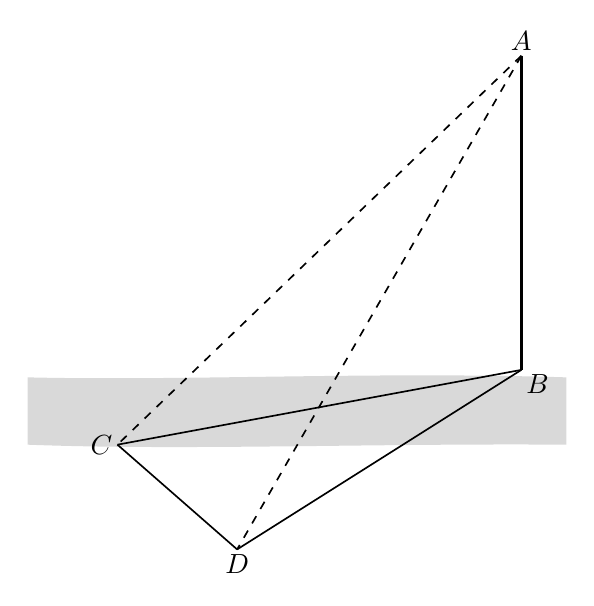
\begin{tikzpicture}[scale=0.95, semithick,
  every node/.style={inner sep=1.5pt}]

  \coordinate (B) at (4.0,1.0);
  \coordinate (A) at (4.0,5.2);
  \coordinate (C) at (-1.4,0.0);
  \coordinate (D) at (0.2,-1.4);

  % 河面（近岸与对岸之间的灰色带）
  \fill[gray!30]
    (-2.6,0.0) .. controls (-0.5,-0.08) and (2.0,0.02) .. (4.6,0.0)
    -- (4.6,0.9) .. controls (2.0,0.98) and (-0.5,0.85) .. (-2.6,0.9) -- cycle;

  % 塔
  \draw[line width=1.1pt] (A) -- (B);
  \node[above] at (A) {$A$};
  \node[below right] at (B) {$B$};

  % 水平基线与视线
  \draw (C) -- (D);
  \draw (B) -- (C);
  \draw (B) -- (D);
  \draw[dashed] (A) -- (C);
  \draw[dashed] (A) -- (D);

  \node[left] at (C) {$C$};
  \node[below] at (D) {$D$};
\end{tikzpicture}
\end{center}
\nopagebreak[4]
\Needspace{4\baselineskip}
\textbf{解析}

\Needspace{5\baselineskip}
在 $\triangle BCD$ 中，

\nopagebreak[4]
\[\angle CBD=180^\circ-\alpha-\beta.\]

\Needspace{5\baselineskip}
由正弦定理，

\nopagebreak[4]
\[\frac{BC}{\sin\angle BDC}=\frac{CD}{\sin\angle CBD},\]

\Needspace{5\baselineskip}
即

\nopagebreak[4]
\[\frac{BC}{\sin\beta}=\frac{s}{\sin(\alpha+\beta)}.\]

\Needspace{5\baselineskip}
故

\nopagebreak[4]
\[BC=\frac{s\sin\beta}{\sin(\alpha+\beta)}.\]

\Needspace{5\baselineskip}
在 $\mathrm{Rt}\triangle ABC$ 中，$AB\perp$ 水平面，$BC$ 在水平面内，$\angle ACB=\theta$，故

\nopagebreak[4]
\[AB=BC\tan\theta=\frac{s\sin\beta\tan\theta}{\sin(\alpha+\beta)}.\]

（判断要点：先在水平面内的 $\triangle BCD$ 中用正弦定理求 $BC$，再在竖直的直角三角形 $ABC$ 中用仰角的正切求塔高；注意 $\angle CBD=180^\circ-\alpha-\beta$。）

\gkanswer{答案：$AB=\dfrac{s\sin\beta\tan\theta}{\sin(\alpha+\beta)}$。}

\end{answer}
\begin{answer}
\gksolhead{18}{}

\textbf{题目}：

如图，在三棱锥 $S-ABC$ 中，侧面 $SAB$ 与侧面 $SAC$ 均为等边三角形，$\angle BAC=90^\circ$，$O$ 为 $BC$ 中点。

（1）证明：$SO\perp$ 平面 $ABC$；

（2）求二面角 $A-SC-B$ 的余弦值。
\nopagebreak[4]
\begin{center}% 2007 年新课标卷理科第 18 题：三棱锥 S-ABC，O 为 BC 中点。
%   侧面 SAB 与 SAC 为等边三角形，∠BAC=90°；SO 为高（虚线）。
% 来源 PDF：gaokaomath-src/普通高考/2007/2007新课标理(海南,宁夏).pdf
% SHA-256：c8ee1632ac3a7a28aab1150f047a2e1c74398ca2944701e9165237897ae724e2
% 原页：2007新课标理(海南,宁夏).pdf 第 1 页（A3 三栏）第 3 栏，书页码 393。
% 重绘依据：按原页顶点位置、虚实线与 O 点位置重绘。
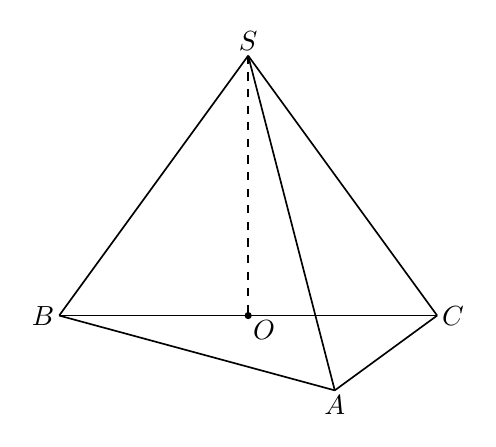
\begin{tikzpicture}[scale=1.0, semithick,
  every node/.style={inner sep=1.5pt}]

  \coordinate (S) at (0,3.3);
  \coordinate (B) at (-2.4,0);
  \coordinate (C) at (2.4,0);
  \coordinate (A) at (1.1,-0.95);
  \coordinate (O) at (0,0);

  \draw (S) -- (A);
  \draw (S) -- (B);
  \draw (S) -- (C);
  \draw (A) -- (B);
  \draw (A) -- (C);
  \draw (B) -- (C);
  \draw[dashed] (S) -- (O);

  \fill (O) circle (1.3pt);
  \node[above] at (S) {$S$};
  \node[left] at (B) {$B$};
  \node[right] at (C) {$C$};
  \node[below] at (A) {$A$};
  \node[below right] at (O) {$O$};
\end{tikzpicture}
\end{center}
\nopagebreak[4]
\Needspace{4\baselineskip}
\textbf{解析}

\Needspace{5\baselineskip}
（1）设

\nopagebreak[4]
\[AB=AC=SA=SB=SC=a.\]

\Needspace{5\baselineskip}
由 $\angle BAC=90^\circ$，$BC=\sqrt2a$，且 $O$ 为 $BC$ 中点，故

\nopagebreak[4]
\[AO=\frac{BC}{2}=\frac{\sqrt2}{2}a.\]

\Needspace{5\baselineskip}
在 $\triangle SBC$ 中，$SB=SC=a$，$BC=\sqrt2a$，故

\nopagebreak[4]
\[SB^2+SC^2=2a^2=BC^2,\]

\Needspace{5\baselineskip}
所以 $\angle BSC=90^\circ$，$SO$ 为斜边中线：

\nopagebreak[4]
\[SO=\frac{BC}{2}=\frac{\sqrt2}{2}a.\]

\Needspace{5\baselineskip}
在 $\triangle SOA$ 中，

\nopagebreak[4]
\[SO^2+AO^2=\frac{a^2}{2}+\frac{a^2}{2}=a^2=SA^2,\]

故 $\angle SOA=90^\circ$，即 $SO\perp AO$。

\Needspace{5\baselineskip}
又 $\triangle SBC$ 为等腰三角形，$O$ 为 $BC$ 中点，故 $SO\perp BC$。$AO$ 与 $BC$ 是平面 $ABC$ 内两条相交直线，所以

\nopagebreak[4]
\[SO\perp\text{\text{平面} }ABC.\]

\Needspace{5\baselineskip}
（2）以 $O$ 为原点，$OA$，$OB$，$OS$ 所在直线分别为 $x$，$y$，$z$ 轴建立空间直角坐标系。不妨取 $a=\sqrt2$，则

\nopagebreak[4]
\[A(1,0,0),\quad B(0,1,0),\quad C(0,-1,0),\quad S(0,0,1).\]

\Needspace{5\baselineskip}
平面 $ASC$ 内，

\nopagebreak[4]
\[\overrightarrow{AC}=(-1,-1,0),\qquad \overrightarrow{AS}=(-1,0,1).\]

\Needspace{5\baselineskip}
取法向量

\nopagebreak[4]
\[\boldsymbol n_1=(1,-1,1),\]

可验证 $\boldsymbol n_1\cdot\overrightarrow{AC}=0$，$\boldsymbol n_1\cdot\overrightarrow{AS}=0$。

\Needspace{5\baselineskip}
平面 $BSC$ 过 $B(0,1,0)$，$C(0,-1,0)$，$S(0,0,1)$，三点 $x$ 坐标都为 $0$，故平面为 $x=0$，法向量取

\nopagebreak[4]
\[\boldsymbol n_2=(1,0,0).\]

\Needspace{5\baselineskip}
于是

\nopagebreak[4]
\[\cos\langle\boldsymbol n_1,\boldsymbol n_2\rangle=\frac{|\boldsymbol n_1\cdot\boldsymbol n_2|}{|\boldsymbol n_1||\boldsymbol n_2|}=\frac{1}{\sqrt3}=\frac{\sqrt3}{3}.\]

\Needspace{5\baselineskip}
由图形知二面角 $A-SC-B$ 为锐角，故其余弦值为

\nopagebreak[4]
\[\frac{\sqrt3}{3}.\]

（判断要点：第（1）问用勾股定理逆定理证 $SO\perp AO$，再结合 $SO\perp BC$；第（2）问建系后平面 $BSC$ 恰为 $x=0$，法向量取 $(1,0,0)$ 最简。）

\gkanswer{答案：（1）证明见解析；（2）$\dfrac{\sqrt3}{3}$。}

\end{answer}
\begin{answer}
\gksolhead{19}{}

\textbf{题目}：

在平面直角坐标系 $xOy$ 中，经过点 $(0,\sqrt2)$ 且斜率为 $k$ 的直线 $l$ 与椭圆 $\dfrac{x^2}{2}+y^2=1$ 有两个不同的交点 $P$ 和 $Q$。

（1）求 $k$ 的取值范围；

（2）设椭圆与 $x$ 轴正半轴、$y$ 轴正半轴的交点分别为 $A$，$B$，是否存在常数 $k$，使得向量 $\overrightarrow{OP}+\overrightarrow{OQ}$ 与 $\overrightarrow{AB}$ 共线？如果存在，求 $k$ 值；如果不存在，请说明理由。

\Needspace{4\baselineskip}
\textbf{解析}

\Needspace{5\baselineskip}
（1）直线 $l$ 的方程为

\nopagebreak[4]
\[y=kx+\sqrt2.\]

\Needspace{5\baselineskip}
代入椭圆

\nopagebreak[4]
\[\frac{x^2}{2}+y^2=1,\]

\Needspace{5\baselineskip}
得

\nopagebreak[4]
\[\frac{x^2}{2}+(kx+\sqrt2)^2=1,\]

\Needspace{5\baselineskip}
即

\nopagebreak[4]
\[\left(\frac12+k^2\right)x^2+2\sqrt2kx+1=0.\]

\Needspace{5\baselineskip}
有两个不同交点，需判别式为正：

\nopagebreak[4]
\[\Delta=(2\sqrt2k)^2-4\left(\frac12+k^2\right)=8k^2-2-4k^2=4k^2-2>0.\]

\Needspace{5\baselineskip}
故

\nopagebreak[4]
\[k^2>\frac12\ \Rightarrow\ k<-\frac{\sqrt2}{2}\ \text{\text{或}}\ k>\frac{\sqrt2}{2}.\]

\Needspace{5\baselineskip}
（2）椭圆与 $x$ 轴正半轴、$y$ 轴正半轴的交点分别为

\nopagebreak[4]
\[A(\sqrt2,0),\qquad B(0,1),\]

\Needspace{5\baselineskip}
故

\nopagebreak[4]
\[\overrightarrow{AB}=(-\sqrt2,1).\]

\Needspace{5\baselineskip}
设 $P(x_1,y_1)$，$Q(x_2,y_2)$。由（1）的方程，

\nopagebreak[4]
\[x_1+x_2=-\frac{2\sqrt2k}{\frac12+k^2}.\]

\Needspace{5\baselineskip}
又 $y_i=kx_i+\sqrt2$，故

\nopagebreak[4]
\[y_1+y_2=k(x_1+x_2)+2\sqrt2=-\frac{2\sqrt2k^2}{\frac12+k^2}+2\sqrt2=\frac{\sqrt2}{\frac12+k^2}.\]

\Needspace{5\baselineskip}
若 $\overrightarrow{OP}+\overrightarrow{OQ}=(x_1+x_2,y_1+y_2)$ 与 $\overrightarrow{AB}=(-\sqrt2,1)$ 共线，则

\nopagebreak[4]
\[\frac{x_1+x_2}{-\sqrt2}=\frac{y_1+y_2}{1}.\]

\Needspace{5\baselineskip}
代入：

\nopagebreak[4]
\[\frac{2k}{\frac12+k^2}=\frac{\sqrt2}{\frac12+k^2},\]

\Needspace{5\baselineskip}
得

\nopagebreak[4]
\[k=\frac{\sqrt2}{2}.\]

但 $k=\dfrac{\sqrt2}{2}$ 时 $\Delta=0$，直线与椭圆只有一个交点，不满足“两个不同的交点”。因此不存在这样的常数 $k$。

（判断要点：第（1）问只需求判别式大于零；第（2）问把共线条件写成坐标比例，解出的 $k$ 必须回到（1）的范围检验，此处恰为边界值，故不存在。）

\gkanswer{答案：（1）$k<-\dfrac{\sqrt2}{2}$ 或 $k>\dfrac{\sqrt2}{2}$；（2）不存在。}

\end{answer}
\begin{answer}
\gksolhead{20}{}

\textbf{题目}：

如图，面积为 $S$ 的正方形 $ABCD$ 中有一个不规则的图形 $M$，可按下面方法估计 $M$ 的面积：在正方形 $ABCD$ 中随机投掷 $n$ 个点，若 $n$ 个点中有 $m$ 个点落入 $M$ 中，则 $M$ 的面积的估计值为 $\dfrac mnS$。假设正方形 $ABCD$ 的边长为 $2$，$M$ 的面积为 $1$，并向正方形 $ABCD$ 中随机投掷 $10000$ 个点，以 $X$ 表示落入 $M$ 中的点的数目。

（1）求 $X$ 的均值 $EX$；

（2）求用以上方法估计 $M$ 的面积时，$M$ 的面积的估计值与实际值之差在区间 $(-0.03,0.03)$ 内的概率。

附表：$P(k)=\sum\limits_{i=0}^{k}\mathrm C_{10000}^i\times0.25^i\times0.75^{10000-i}$

\begin{center}
\begin{tabular}{lllll}
\toprule
$k$ & $2424$ & $2425$ & $2574$ & $2575$ \\
\midrule
$P(k)$ & $0.0403$ & $0.0423$ & $0.9570$ & $0.9590$ \\
\bottomrule
\end{tabular}
\end{center}
\nopagebreak[4]
\begin{center}% 2007 年新课标卷理科第 20 题：正方形 ABCD 内的不规则图形 M。
% 来源 PDF：gaokaomath-src/普通高考/2007/2007新课标理(海南,宁夏).pdf
% SHA-256：c8ee1632ac3a7a28aab1150f047a2e1c74398ca2944701e9165237897ae724e2
% 原页：2007新课标理(海南,宁夏).pdf 第 2 页（A3 三栏）第 1 栏，书页码 394。
% 重绘依据：按原页正方形的顶点标注与内部不规则阴影轮廓重绘，轮廓为示意。
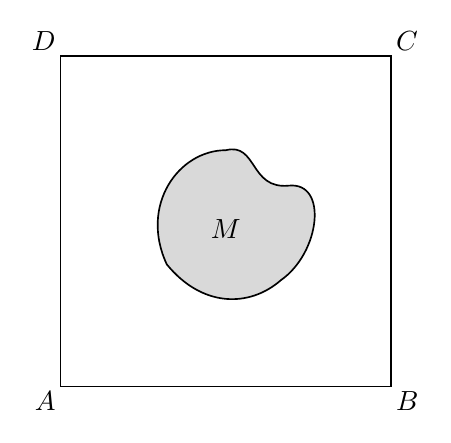
\begin{tikzpicture}[scale=1.0, semithick,
  every node/.style={inner sep=1.5pt}]

  \draw (0,0) rectangle (4.2,4.2);
  \node[below left] at (0,0) {$A$};
  \node[below right] at (4.2,0) {$B$};
  \node[above right] at (4.2,4.2) {$C$};
  \node[above left] at (0,4.2) {$D$};

  \fill[gray!30]
    (1.35,1.55) .. controls (1.0,2.3) and (1.5,3.0) ..
    (2.1,3.0) .. controls (2.5,3.1) and (2.4,2.5) ..
    (2.9,2.55) .. controls (3.4,2.6) and (3.3,1.7) ..
    (2.8,1.35) .. controls (2.4,1.0) and (1.8,1.0) ..
    (1.35,1.55) -- cycle;
  \draw
    (1.35,1.55) .. controls (1.0,2.3) and (1.5,3.0) ..
    (2.1,3.0) .. controls (2.5,3.1) and (2.4,2.5) ..
    (2.9,2.55) .. controls (3.4,2.6) and (3.3,1.7) ..
    (2.8,1.35) .. controls (2.4,1.0) and (1.8,1.0) ..
    (1.35,1.55) -- cycle;
  \node at (2.1,2.0) {$M$};
\end{tikzpicture}
\end{center}
\nopagebreak[4]
\Needspace{4\baselineskip}
\textbf{解析}

\Needspace{5\baselineskip}
（1）正方形面积为 $4$，$M$ 的面积为 $1$，故随机投一点落入 $M$ 的概率为

\nopagebreak[4]
\[p=\frac14.\]

\Needspace{5\baselineskip}
投掷 $10000$ 个点，$X$ 服从二项分布，故

\nopagebreak[4]
\[EX=10000\times\frac14=2500.\]

\Needspace{5\baselineskip}
（2）$M$ 面积的估计值为

\nopagebreak[4]
\[\hat S=\frac{X}{10000}\times4=\frac{X}{2500}.\]

\Needspace{5\baselineskip}
要求估计值与实际值之差在 $(-0.03,0.03)$ 内：

\nopagebreak[4]
\[\left|\frac{X}{2500}-1\right|<0.03.\]

\Needspace{5\baselineskip}
即

\nopagebreak[4]
\[-0.03<\frac{X}{2500}-1<0.03\ \Rightarrow\ 2425<X<2575.\]

\Needspace{5\baselineskip}
$X$ 为整数，故 $X=2426,2427,\cdots,2574$。于是

\nopagebreak[4]
\[P=P(X\leqslant2574)-P(X\leqslant2425).\]

\Needspace{5\baselineskip}
查表：

\nopagebreak[4]
\[P(2574)=0.9570,\qquad P(2425)=0.0423,\]

\Needspace{5\baselineskip}
故

\nopagebreak[4]
\[P=0.9570-0.0423=0.9147.\]

（判断要点：估计值 $\hat S=\dfrac{X}{10000}\times4$，不要直接用 $\dfrac{X}{10000}$；区间端点 $2425$ 与 $2575$ 都使差恰为 $\pm0.03$，应排除，所以用 $P(2574)-P(2425)$。）

\gkanswer{答案：（1）$2500$；（2）$0.9147$。}

\end{answer}
\begin{answer}
\gksolhead{21}{}

\textbf{题目}：

设函数 $f(x)=\ln(x+a)+x^2$。

（1）若当 $x=-1$ 时，$f(x)$ 取得极值，求 $a$ 的值，并讨论 $f(x)$ 的单调性；

（2）若 $f(x)$ 存在极值，求 $a$ 的取值范围，并证明所有极值之和大于 $\ln\dfrac{\mathrm e}{2}$。

\Needspace{4\baselineskip}
\textbf{解析}

\Needspace{5\baselineskip}
（1）

\nopagebreak[4]
\[f'(x)=\frac1{x+a}+2x.\]

\Needspace{5\baselineskip}
由 $x=-1$ 时取得极值，

\nopagebreak[4]
\[f'(-1)=\frac1{a-1}-2=0\ \Rightarrow\ a-1=\frac12\ \Rightarrow\ a=\frac32.\]

\Needspace{5\baselineskip}
此时定义域为 $x>-\dfrac32$，且

\nopagebreak[4]
\[f'(x)=\frac1{x+\frac32}+2x=\frac{2x^2+3x+1}{x+\frac32}=\frac{(2x+1)(x+1)}{x+\frac32}.\]

分子零点为 $x=-1$ 与 $x=-\dfrac12$，分母恒正。列表：

\begin{itemize}
\item $-\dfrac32<x<-1$ 时，$f'(x)>0$，$f$ 递增；
\item $-1<x<-\dfrac12$ 时，$f'(x)<0$，$f$ 递减；
\item $x>-\dfrac12$ 时，$f'(x)>0$，$f$ 递增。
\end{itemize}

故增区间为 $\left(-\dfrac32,-1\right)$ 与 $\left(-\dfrac12,+\infty\right)$，减区间为 $\left(-1,-\dfrac12\right)$。

\Needspace{5\baselineskip}
（2）

\nopagebreak[4]
\[f'(x)=0\ \Leftrightarrow\ \frac1{x+a}+2x=0\ \Leftrightarrow\ 2x^2+2ax+1=0\quad(x>-a).\]

\Needspace{5\baselineskip}
方程有实根需

\nopagebreak[4]
\[\Delta=4a^2-8>0\ \Rightarrow\ a>\sqrt2\ \text{\text{或}}\ a<-\sqrt2.\]

\Needspace{5\baselineskip}
当 $a<-\sqrt2$ 时，两根

\nopagebreak[4]
\[x_{1,2}=\frac{-a\pm\sqrt{a^2-2}}{2}\]

都小于 $-a$（因为 $\sqrt{a^2-2}<-a$），不在定义域 $x>-a$ 内，此时 $f'(x)>0$ 恒成立，无极值。

\Needspace{5\baselineskip}
当 $a>\sqrt2$ 时，两根

\nopagebreak[4]
\[x_1=\frac{-a-\sqrt{a^2-2}}{2},\qquad x_2=\frac{-a+\sqrt{a^2-2}}{2}\]

\Needspace{5\baselineskip}
都大于 $-a$，且 $f'$ 在两根间变号，故有两个极值。于是 $a$ 的取值范围是

\nopagebreak[4]
\[a>\sqrt2.\]

\Needspace{5\baselineskip}
极值之和为

\nopagebreak[4]
\[f(x_1)+f(x_2)=\ln(x_1+a)+x_1^2+\ln(x_2+a)+x_2^2.\]

\Needspace{5\baselineskip}
由韦达定理，

\nopagebreak[4]
\[x_1+x_2=-a,\qquad x_1x_2=\frac12,\]

\Needspace{5\baselineskip}
故

\nopagebreak[4]
\[(x_1+a)(x_2+a)=x_1x_2+a(x_1+x_2)+a^2=\frac12,\]

\nopagebreak[4]
\[x_1^2+x_2^2=(x_1+x_2)^2-2x_1x_2=a^2-1.\]

\Needspace{5\baselineskip}
于是极值之和为

\nopagebreak[4]
\[f(x_1)+f(x_2)=\ln\frac12+a^2-1=a^2-1-\ln2.\]

\Needspace{5\baselineskip}
因为 $a>\sqrt2$，所以 $a^2>2$，从而

\nopagebreak[4]
\[a^2-1-\ln2>2-1-\ln2=1-\ln2=\ln\frac{\mathrm e}{2}.\]

（判断要点：第（2）问先由判别式得 $|a|>\sqrt2$，再检验两根是否落在定义域内，排除 $a<-\sqrt2$；极值之和用韦达定理化简，$(x_1+a)(x_2+a)=\dfrac12$ 是消去对数项的关键。）

\gkanswer{答案：（1）$a=\dfrac32$，增区间 $\left(-\dfrac32,-1\right)$，$\left(-\dfrac12,+\infty\right)$，减区间 $\left(-1,-\dfrac12\right)$；（2）$a>\sqrt2$。}

\end{answer}
\begin{answer}
\gksolhead{22}{}

\textbf{题目}：

如图，已知 $AP$ 是 $\odot O$ 的切线，$P$ 为切点，$AC$ 是 $\odot O$ 的割线，与 $\odot O$ 交于 $B$，$C$ 两点，圆心 $O$ 在 $\angle PAC$ 的内部，点 $M$ 是 $BC$ 的中点。

（1）证明 $A$，$P$，$O$，$M$ 四点共圆；

（2）求 $\angle OAM+\angle APM$ 的大小。
\nopagebreak[4]
\begin{center}% 2007 年新课标卷理科第 22 题：圆的切线 AP、割线 ABC、弦 BC 中点 M。
%   圆 O 半径 2，A(-4,0)，切点 P=(-1,√3)；
%   割线 ABC 从 A 出发，B、C 为与圆的交点，M 为 BC 中点。
% 来源 PDF：gaokaomath-src/普通高考/2007/2007新课标理(海南,宁夏).pdf
% SHA-256：c8ee1632ac3a7a28aab1150f047a2e1c74398ca2944701e9165237897ae724e2
% 原页：2007新课标理(海南,宁夏).pdf 第 2 页（A3 三栏）第 3 栏，书页码 394。
% 重绘依据：按原页点、线与圆的位置重绘；A-O 与 P-M 为题目用到的辅助线。
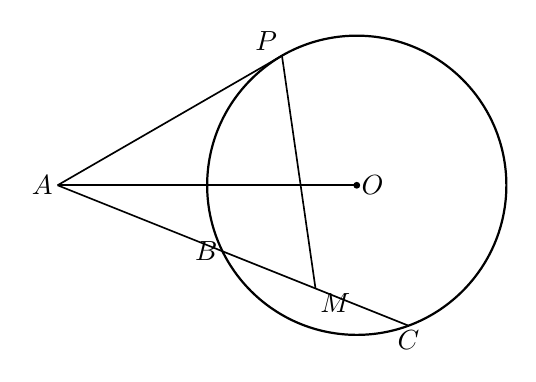
\begin{tikzpicture}[scale=0.95, semithick,
  every node/.style={inner sep=1.5pt}]

  \coordinate (O) at (0,0);
  \coordinate (A) at (-4,0);
  \coordinate (P) at (-1,1.732);
  \coordinate (B) at (-1.795,-0.882);
  \coordinate (C) at (0.692,-1.877);
  \coordinate (M) at (-0.5515,-1.3795);

  \draw[thick] (O) circle (2);
  \fill (O) circle (1.3pt);

  % 切线、割线与辅助线
  \draw (A) -- (P);
  \draw (A) -- (C);
  \draw (A) -- (O);
  \draw (P) -- (M);

  \node[left] at (A) {$A$};
  \node[above left] at (P) {$P$};
  \node[right] at (O) {$O$};
  \node[left] at (B) {$B$};
  \node[below] at (C) {$C$};
  \node[below right] at (M) {$M$};
\end{tikzpicture}
\end{center}
\nopagebreak[4]
\Needspace{4\baselineskip}
\textbf{解析}

\Needspace{5\baselineskip}
（1）$AP$ 是 $\odot O$ 的切线，$P$ 为切点，故

\nopagebreak[4]
\[OP\perp AP\ \Rightarrow\ \angle OPA=90^\circ.\]

\Needspace{5\baselineskip}
$M$ 是弦 $BC$ 的中点，故

\nopagebreak[4]
\[OM\perp BC.\]

\Needspace{5\baselineskip}
又 $A$，$B$，$M$，$C$ 在同一直线上，所以 $OM\perp AM$，即

\nopagebreak[4]
\[\angle OMA=90^\circ.\]

于是 $P$ 与 $M$ 都在以 $AO$ 为直径的圆上（直径所对的圆周角为直角），故 $A$，$P$，$O$，$M$ 四点共圆。

\Needspace{5\baselineskip}
（2）由（1），$A$，$P$，$O$，$M$ 四点共圆，$\angle APM$ 与 $\angle AOM$ 都是弧 $AM$ 所对的圆周角，故

\nopagebreak[4]
\[\angle APM=\angle AOM.\]

\Needspace{5\baselineskip}
于是

\nopagebreak[4]
\[\angle OAM+\angle APM=\angle OAM+\angle AOM.\]

\Needspace{5\baselineskip}
在 $\triangle AOM$ 中，$\angle AMO=90^\circ$，故

\nopagebreak[4]
\[\angle OAM+\angle AOM=90^\circ.\]

\Needspace{5\baselineskip}
所以

\nopagebreak[4]
\[\angle OAM+\angle APM=90^\circ.\]

（判断要点：证明四点共圆用“以 $AO$ 为直径的圆”；第（2）问用同弧所对的圆周角相等，把 $\angle APM$ 换成 $\angle AOM$，再在直角三角形 $AOM$ 中求和。）

\gkanswer{答案：（1）证明见解析；（2）$90^\circ$。}

\end{answer}
\begin{answer}
\gksolhead{23}{}

\textbf{题目}：

$\odot O_1$ 和 $\odot O_2$ 的极坐标方程分别为 $\rho=4\cos\theta$，$\rho=-4\sin\theta$。

（1）把 $\odot O_1$ 和 $\odot O_2$ 的极坐标方程化为直角坐标方程；

（2）求经过 $\odot O_1$，$\odot O_2$ 交点的直线的直角坐标方程。

\Needspace{4\baselineskip}
\textbf{解析}

\Needspace{5\baselineskip}
（1）由 $\rho=4\cos\theta$，两边乘 $\rho$：

\nopagebreak[4]
\[\rho^2=4\rho\cos\theta.\]

\Needspace{5\baselineskip}
利用 $\rho^2=x^2+y^2$，$\rho\cos\theta=x$，得

\nopagebreak[4]
\[x^2+y^2=4x,\]

\Needspace{5\baselineskip}
配方：

\nopagebreak[4]
\[(x-2)^2+y^2=4.\]

\Needspace{5\baselineskip}
由 $\rho=-4\sin\theta$，两边乘 $\rho$：

\nopagebreak[4]
\[\rho^2=-4\rho\sin\theta,\]

\Needspace{5\baselineskip}
即

\nopagebreak[4]
\[x^2+y^2=-4y,\]

\Needspace{5\baselineskip}
配方：

\nopagebreak[4]
\[x^2+(y+2)^2=4.\]

\Needspace{5\baselineskip}
（2）两圆方程分别为

\nopagebreak[4]
\[x^2+y^2-4x=0,\qquad x^2+y^2+4y=0.\]

\Needspace{5\baselineskip}
相减：

\nopagebreak[4]
\[-4x-4y=0\ \Rightarrow\ x+y=0.\]

这就是经过两圆交点的直线（公共弦）的直角坐标方程。

（判断要点：极坐标化直角坐标时两边乘 $\rho$ 是关键；两圆方程相减直接得到公共弦所在直线。）

\gkanswer{答案：（1）$(x-2)^2+y^2=4$，$x^2+(y+2)^2=4$；（2）$x+y=0$。}

\end{answer}
\begin{answer}
\gksolhead{24}{}

\textbf{题目}：

设函数 $f(x)=|2x+1|-|x-4|$。

（1）解不等式 $f(x)>2$；

（2）求函数 $y=f(x)$ 的最小值。

\Needspace{4\baselineskip}
\textbf{解析}

先分三段去掉绝对值。零点为 $x=-\dfrac12$ 与 $x=4$。

\Needspace{5\baselineskip}
当 $x<-\dfrac12$ 时，

\nopagebreak[4]
\[f(x)=-(2x+1)+(x-4)=-x-5;\]

\Needspace{5\baselineskip}
当 $-\dfrac12\leqslant x<4$ 时，$|2x+1|=2x+1$，$|x-4|=4-x$，故

\nopagebreak[4]
\[f(x)=2x+1-(4-x)=3x-3;\]

\Needspace{5\baselineskip}
当 $x\geqslant4$ 时，

\nopagebreak[4]
\[f(x)=2x+1-(x-4)=x+5.\]

\Needspace{5\baselineskip}
即

\nopagebreak[4]
\[f(x)=\begin{cases}-x-5,&x<-\dfrac12,\\ 3x-3,&-\dfrac12\leqslant x<4,\\ x+5,&x\geqslant4.\end{cases}\]

（1）解 $f(x)>2$：

\begin{itemize}
\item $x<-\dfrac12$ 时，$-x-5>2$，得 $x<-7$；
\item $-\dfrac12\leqslant x<4$ 时，$3x-3>2$，得 $x>\dfrac53$，即 $\dfrac53<x<4$；
\item $x\geqslant4$ 时，$x+5>2$ 恒成立，即 $x\geqslant4$。
\end{itemize}

\Needspace{5\baselineskip}
合并得

\nopagebreak[4]
\[x<-7\ \text{\text{或}}\ x>\frac53.\]

（2）各段的最小值：

\begin{itemize}
\item $x<-\dfrac12$ 时，$-x-5>-\dfrac92$；
\item $-\dfrac12\leqslant x<4$ 时，$3x-3\geqslant3\times\left(-\dfrac12\right)-3=-\dfrac92$；
\item $x\geqslant4$ 时，$x+5\geqslant9$。
\end{itemize}

\Needspace{5\baselineskip}
故最小值为

\nopagebreak[4]
\[f\left(-\frac12\right)=-\frac92.\]

（判断要点：分段去绝对值时，$|x-4|$ 在 $x<4$ 时为 $4-x$；第（2）问在各段上分别求最小值再比较，最小值在分界点 $x=-\dfrac12$ 取到。）

\gkanswer{答案：（1）$x<-7$ 或 $x>\dfrac53$；（2）$-\dfrac92$。}

\end{answer}